\chapter{Ownership, Cost, and the Discipline of Scale}

This lecture opens the way many interviews about wealth do: by flashing scale before it explains structure. We hear of a musician with a \$25 million year, a beverage founder doing annual sales measured in billions, a company at roughly \$12 billion in revenue and roughly \$25 billion in valuation, and a mayor governing \(8.5\times 10^6\) people. Then the lecture slows down. What matters is not the spectacle by itself, but the mechanism hidden underneath it. As the host moves through New York and then out to Long Island, we are led through four distinct machines of wealth: own the asset, control the cost base, build with the right people, and keep the next step available even under pressure.

\section{New York as a Field of Wealth}

The first honest fact in the lecture is not financial. It is social. Wealth is visible in New York, but explanation is scarce. The host walks the streets, asks direct questions, and gets fragments in return: a joke, an evasion, a reminder that some people are private, a quick remark about having been ``born in the right place.'' The city is rich, but it does not volunteer its operating principles.

That matters because the lecture is carefully staged. It does not begin with a doctrine of wealth. It begins with access friction. Before we are allowed to see a balance sheet, we are asked to notice how hard it is to stop the people who might have one. The host then says, in effect, that Manhattan is the wrong local geometry for the interview he wants, and so the lecture changes place. It takes the train to Tribeca. That shift is not decorative. It is the first real transition in the argument: if explanation is withheld in one part of the city, then the lecture must move until a speaker appears who can make the hidden structure visible.

The cold-open montage is useful precisely because it plants a set of scale markers before any mechanism is given. Later, as the lecture unfolds, those numbers become more stable:
\begin{align}
R_{\mathrm{Russ,yr}} &\approx \$25\times 10^6,\\
R_{\mathrm{Arizona,yr}} &< \$3\times 10^9,\\
R_{\mathrm{Fanatics}} &\approx \$12\times 10^9,\\
N_{\mathrm{NYC}} &= 8.5\times 10^6.
\end{align}
We do not yet know what generates these scales. The rest of the chapter is the answer to that question.

\section{Owning the Music, Not Just Making It}

In Tribeca the lecture finds Russ, and the first serious mechanism arrives almost immediately. The surprise is not only that a musician can be rich. The surprise is that the explanation is phrased so cleanly. Most musicians, he says, do not end up rich because they do not own their music. In one stroke the lecture shifts us from celebrity to asset structure.

\begin{definition}
In the language of this lecture, the \emph{master} is the owned sound recording. It is the revenue-bearing object. To give away the master is not merely to give away a performance; it is to transfer the claim on future cash flow.
\end{definition}

Once we have that definition, the next step is nearly forced. A catalog of owned masters behaves differently from a career built on a single breakout song. The lecture gives only an approximate count, but the mechanism is clear:
\begin{equation}
I_{\mathrm{catalog}}=\sum_{i=1}^{N} I_i,\qquad N\approx 500+.
\end{equation}
This is the simplest important equation in the chapter. One song is a lottery ticket. Hundreds of owned songs form a catalog, and a catalog is a machine for converting repeated listening into repeated revenue. Russ says exactly this in ordinary language: he does not need one song to make him a million dollars if he has hundreds of songs each making some smaller amount. That is diversification, but diversification of owned creative property.

The host then asks the obvious follow-up. If music can do this, why do so many artists remain broke?

\subsection{Question \& Answer}

\paragraph{Question.} If music makes money, why are so many musicians broke?

\paragraph{Answer.} Because the artist and the asset are not identical. The lecture answers by passing through a simple recoupment story. A label advances money up front, but the advance is not a gift. It creates a threshold:
\begin{align}
A &= \$2\,\mathrm{M},\\
R_{\mathrm{music}}<A &\Longrightarrow n_{\mathrm{checks}}=0,\\
R_{\mathrm{music}}\ge A &\Longrightarrow R_{\mathrm{post}}=R_{\mathrm{music}}-A,\\
R_{\mathrm{artist}} &\approx \frac{1}{2}R_{\mathrm{post}}.
\end{align}
Here \(A\) is the advance, \(R_{\mathrm{music}}\) is the cumulative revenue returned by the music, \(R_{\mathrm{post}}\) is the revenue remaining after recoupment, and \(n_{\mathrm{checks}}\) is the number of later royalty checks in the lecture's simplified picture. The split is illustrative rather than universal, but the threshold logic is the point.

If the music never earns back the advance, then the artist remains unrecouped and the later checks do not arrive. If the advance is earned back, then only the post-recoupmment flow is actually shareable. Russ summarizes the timing in the plainest possible way: if you are recouped, you get two checks a year. If you are not, then even that thin periodic flow disappears.

\begin{figure}
\centering
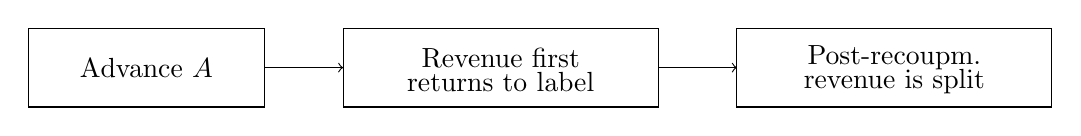
\begin{tikzpicture}[x=1cm,y=1cm]
\draw (0,0) rectangle (3,1);
\node at (1.5,0.5) {Advance \(A\)};
\draw[->] (3,0.5) -- (4,0.5);
\draw (4,0) rectangle (8,1);
\node at (6,0.62) {Revenue first};
\node at (6,0.32) {returns to label};
\draw[->] (8,0.5) -- (9,0.5);
\draw (9,0) rectangle (13,1);
\node at (11,0.62) {Post-recoupm.};
\node at (11,0.32) {revenue is split};
\end{tikzpicture}
\caption{A transcript-backed recoupment sketch. The lecture's point is simple: the advance is paid back first, and only then does the artist participate in the later flow.}
\end{figure}

That is why Russ becomes so emphatic when he says that the money is in music, and then sharpens the phrase: the money is in \emph{owning} the music. The labels themselves are the evidence. They do not need to tour in order to make money from the recordings they own.

\section{Patience, Public Opinion, and the Artist's Cash-Flow Machine}

At this point the lecture could have stopped with ownership. It does not. Instead it widens from contract structure to the moral and temporal conditions required to preserve ownership. Russ says he turned down \$50 million for the rights to his music. That sentence is placed very carefully in the interview. Ownership is first established as the mechanism; only then does the refusal of a lump sum begin to make sense.

His explanation for the refusal is partly moral and partly economic. He describes selling the rights as a kind of selling of the soul, because the music is not merely a product but an extension of the self. One need not adopt the exact moral language to see the underlying structure. A large lump sum competes against a long-lived stream of owned income. The speaker refuses present certainty in order to preserve future control.

From there the lecture moves, quite naturally, into time. ``Faith requires more than 48 hours'' is not a mystical statement in context. It is a rule about evaluation windows:
\begin{equation}
48\,\mathrm{hours}<1\,\mathrm{week}<1\,\mathrm{year}<2\,\mathrm{years}<10\,\mathrm{years}.
\end{equation}
We are being taught not only to own the asset, but also to refuse early judgment about the asset's value. The shorter the clock, the more likely we are to misread the work.

That argument becomes sharper when Russ turns to reinvestment. He says that the best investment he has ever seen is the music itself, and the lecture provides a compact numerical example.

\paragraph{Worked example.} The transcript gives us a song uploaded for roughly \$9.99 and later reported to have made roughly \$2 million:
\begin{align}
C_{\mathrm{song}} &\approx \$9.99,\\
R_{\mathrm{song}} &\approx \$2{,}000{,}000,\\
\frac{R_{\mathrm{song}}}{C_{\mathrm{song}}} &\sim 2\times 10^5.
\end{align}
This is not audited net profit, and the lecture does not pretend that it is. It is an interview-level order-of-magnitude claim. But that is enough. The point is that an artist who owns the recording and knows how to make the recording already possesses the highest-return reinvestment target inside the business.

The host then asks the next sharp question, and again the lecture answers by drawing a distinction.

\subsection{Question \& Answer}

\paragraph{Question.} How do we survive hate in a business where public feeling is part of the revenue model?

\paragraph{Answer.} By understanding that music is not evaluated like sports. Russ's comparison is illuminating because it marks the boundary between finite performance and approval-dependent performance. In sports, the stat line is objective enough to carry the contract. In music, livelihood is partly a function of how people feel:
\begin{equation}
\mathbf{s}_{\mathrm{sport}}=(25,10,6),\qquad I_{\mathrm{artist}}=F\!\left(P_{\mathrm{public}}\right).
\end{equation}
The right-hand side is deliberately schematic. The lecture does not give us a closed form for \(F\), nor could it. What it gives us is the correct dependence. \(P_{\mathrm{public}}\) is not a box score. It is a social variable: reputation, identification, mood, approval, curiosity.

That is why the lecture explicitly rejects a comforting but false slogan. It is not true that an artist can simply stop caring what anyone thinks. In this line of work, public feeling enters the cash-flow machine. But the answer is not paralysis. It is iteration. Keep releasing. Keep building the catalog. The lecture's operational advice is blunt and memorable: if hate comes, drop your way through it.

The host briefly recaps the interview here in language of astonishment, and that recap matters. It marks the closure of one machine before the lecture moves to a very different one.

\section{Price Power without Debt: The Arizona Machine}

The scene changes from Tribeca to Long Island, and with the change of place the texture of the lecture changes as well. We leave intangible music rights and enter the world of shelves, cans, freight, buildings, and factory bolts. The opening beats of the Don Vultaggio interview preserve the lecture's pattern of astonishment. Arnold Palmer is introduced not as a beverage on a shelf, but as a product created by the man sitting in front of us. Annual sales are pushed toward the billion-dollar scale. Only then does the lecture ask the origin question.

That origin is modest: no family money, no college, truck driving, a small business becoming a larger one over decades. The lecture then reaches backward through Don's father to A\&P and turns a family memory into a commercial warning:
\begin{equation}
S_{\mathrm{A\&P}}:15000\to 0.
\end{equation}
The message is that scale alone is not a shield. A company can be enormous and still disappear if it forgets the customer.

The famous local puzzle then appears in its natural place. Arizona kept a \(99\)-cent product alive for decades. Why?

\subsection{Question \& Answer}

\paragraph{Question.} How can a \(99\)-cent product survive inflation for decades?

\paragraph{Answer.} Because price is not an isolated number. It sits on top of a cost structure and a capital structure. The lecture writes this logic in spoken rather than formal terms, but the algebra is straightforward:
\begin{equation}
\Pi=(p-c)q,\qquad p=\$0.99.
\end{equation}
If \(p\) is to remain low, then \(c\) must be made compatible with that choice. So the lecture decomposes \(c\) into the pieces that matter for the story being told:
\begin{equation}
c=c_{\mathrm{operations}}+c_{\mathrm{distribution}}+c_{\mathrm{interest}}.
\end{equation}
Don's essential claim is that Arizona has driven the financing term to zero:
\begin{equation}
c_{\mathrm{interest}}=0.
\end{equation}
The buildings are owned. The factories are owned. The equipment is owned. There is no bank and no board forcing the price upward merely to service leverage. The miracle of the \(99\)-cent can dissolves once we see that the company is built underneath the retail price in a different way.

\paragraph{Worked derivation.} The lecture's logic can be written as a short commercial derivation.
\begin{enumerate}
\item Hold the retail price at \(p=\$0.99\).
\item Remove financing drag by setting \(c_{\mathrm{interest}}=0\).
\item Reduce the pressure on the unit margin \(p-c\).
\item Accept that the margin may still be thinner than that of a higher-priced rival.
\item Raise or preserve volume \(q\) so that the total profit remains viable.
\end{enumerate}
This is exactly the logic Don invokes when he says that sometimes increased sales can make up for lower margins.

The interview then gives a second numerical marker. A New Jersey factory cost more than \$400 million and was paid for in cash:
\begin{equation}
K_{\mathrm{factory}}>\$4\times 10^8.
\end{equation}
Again the point is not simply that the company is profitable. The point is that retained capital creates strategic freedom.

\begin{figure}
\centering
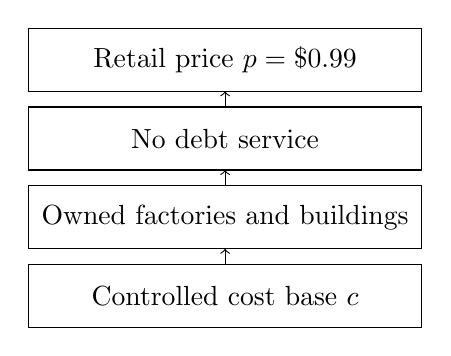
\begin{tikzpicture}[x=1cm,y=1cm]
\draw (0,0) rectangle (5,0.8);
\node at (2.5,0.4) {Retail price \(p=\$0.99\)};
\draw (0,-1) rectangle (5,-0.2);
\node at (2.5,-0.6) {No debt service};
\draw (0,-2) rectangle (5,-1.2);
\node at (2.5,-1.6) {Owned factories and buildings};
\draw (0,-3) rectangle (5,-2.2);
\node at (2.5,-2.6) {Controlled cost base \(c\)};
\draw[->] (2.5,-0.2) -- (2.5,0);
\draw[->] (2.5,-1.2) -- (2.5,-1);
\draw[->] (2.5,-2.2) -- (2.5,-2);
\end{tikzpicture}
\caption{A transcript-backed cost-stack sketch for Arizona. The cheap retail number is supported from below by ownership and debt avoidance.}
\end{figure}

The lecture then widens again. Packaging is the acquisition surface. If Coke and Pepsi can outspend us in conventional advertising, then the container must become the advertisement. People buy with their eyes at the cooler, and the lecture is explicit that this is not an optional flourish. It is how a smaller entrant survives.

Operational modernization enters next. The business doubled in ten years without doubling staff, so productivity must have improved:
\begin{equation}
Y_{10}\approx 2Y_0,\qquad L_{10}<2L_0
\quad\Longrightarrow\quad
\left(\frac{Y}{L}\right)_{10}>\left(\frac{Y}{L}\right)_0.
\end{equation}
We are not given exact output units, but we do not need them. The direction of change is enough. Output per worker rose.

Finally the lecture compresses the entire Arizona section into a primitive but serious law: know your costs and sell above them. The statement sounds simple because it is simple. The warning underneath it is that many businesses fail without ever having actually computed their own unit economics correctly.

\begin{remark}
The video pauses here for a promotional interlude. Since it does not introduce a new mechanism of wealth creation, we set it aside and return to the next substantive interview.
\end{remark}

\section{Rebuilding from Zero: Voids, People, and Relationship Capital}

When the lecture returns to New York, the scale jumps again. Michael Rubin is introduced through familiar spectacle: Fanatics at roughly \$12 billion in revenue, roughly \(22{,}000\) people, and roughly \$25 billion in valuation:
\begin{equation}
R_{\mathrm{Fanatics}}\approx \$12\times 10^9,\qquad
L_{\mathrm{Fanatics}}=22000,\qquad
V_{\mathrm{Fanatics}}\approx \$25\times 10^9.
\end{equation}
But the lecture does something more interesting than admire the number. It immediately sets that number under a hypothetical: if everything were lost tomorrow, how would one rebuild?

Before answering, Rubin restores an important motivational beat. He says he would love the reset. That line matters. It tells us that the lecture is not merely going to describe existing scale. It is going to treat entrepreneurial construction as a repeatable operator.

\subsection{Question \& Answer}

\paragraph{Question.} What are the first moves if we had to rebuild a billion-dollar company from scratch?

\paragraph{Answer.} Rubin gives the cleanest ordered process in the lecture:
\begin{equation}
\text{study}\to\text{find void}\to\text{sprint}\to\text{get the right people}\to\text{iterate after failure}.
\end{equation}
This is not ornamental. It is the lecture's most explicit entrepreneurial algorithm. It begins with attention, not with capital. Study until a market absence becomes visible. Then move quickly. But speed alone is not enough; the process is social. Get the right people because no large business is built alone. If the first attempt fails, run the sequence again.

\begin{figure}
\centering
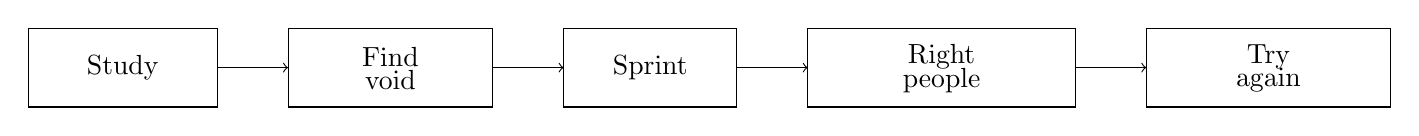
\begin{tikzpicture}[x=1cm,y=1cm]
\draw (0,0) rectangle (2.4,1);
\node at (1.2,0.5) {Study};
\draw[->] (2.4,0.5) -- (3.3,0.5);
\draw (3.3,0) rectangle (5.9,1);
\node at (4.6,0.64) {Find};
\node at (4.6,0.34) {void};
\draw[->] (5.9,0.5) -- (6.8,0.5);
\draw (6.8,0) rectangle (9,1);
\node at (7.9,0.5) {Sprint};
\draw[->] (9,0.5) -- (9.9,0.5);
\draw (9.9,0) rectangle (13.3,1);
\node at (11.6,0.64) {Right};
\node at (11.6,0.34) {people};
\draw[->] (13.3,0.5) -- (14.2,0.5);
\draw (14.2,0) rectangle (17.3,1);
\node at (15.75,0.64) {Try};
\node at (15.75,0.34) {again};
\end{tikzpicture}
\caption{A transcript-backed reconstruction of Rubin's rebuild-from-zero sequence.}
\end{figure}

What follows in the interview is the social underside of that operator. Relationships, Rubin says, do not matter much in good times, but in bad times they matter enormously. This is not conventional networking advice. It is a statement about survival across discontinuity. Relationships carry a company through the interval in which its numbers are not yet impressive and its position is not yet secure.

That is why the lecture keeps pressing on help. Rubin names mentors and allies not as ornaments but as inputs. Robert Kraft and Jonathan Kraft are offered as examples of people who invested time and credibility before the company was fully formed. The lesson is not celebrity proximity. The lesson is that serious scale is almost always socially scaffolded.

The same logic governs his discussion of failure. Broke at fifteen, creditors at the door, then a much larger business a few years later. The transcript garbles the industry name, but not the sequence: by twenty-one he describes himself as doing roughly \$100 million in sales and roughly \$10 million in annual earnings. The point is not to romanticize chaos. The point is to make failure computationally useful. Each loss becomes training data for the next attempt.

That is why the lecture ends this section by stretching the horizon. The host raises the one-year question; Rubin rejects it. The decade is already too short for him:
\begin{equation}
1\,\mathrm{year}<10\,\mathrm{years}<\text{lifetime horizon}.
\end{equation}
The stronger claim here is not moral but structural. Short-term thinking tempts the builder into avoidable mistakes. Lifetime thinking changes the objective from immediate extraction to endurance, reputation, and belovedness after the founder is gone.

\section{One Day at a Time Under Public Pressure}

The final movement of the lecture leaves company-building and enters public leadership. Eric Adams is introduced not as a capitalist operator but as the executive of a city. The arithmetic therefore changes:
\begin{equation}
N_{\mathrm{people}}=8.5\times 10^6,\qquad
N_{\mathrm{opinions}}=3.5\times 10^7.
\end{equation}
The second number is plainly rhetorical, but that is part of its function. It tells us that the mayor's problem is not merely population. It is noise.

Adams first answers the pressure question by shrinking the authority of public judgment. New Yorkers will criticize. They will laugh. They will doubt. One cannot let the middle finger become the governing variable. That answer leads directly into his most memorable line about haters becoming waiters at the table of success. The rhythm here matters. The lecture moves from outer noise to inner steadiness before it ever reaches the deeper autobiographical material.

Only then does Adams speak of dyslexia, ridicule, bullying, and the systems he had to build in order to function well. The lecture's metaphor of dark places as plantings is important because it changes the interpretation of adversity. The bad beginning is not erased. It is reassigned a different role.

\subsection{Question \& Answer}

\paragraph{Question.} What is the first actionable step when we are at rock bottom?

\paragraph{Answer.} Adams's answer is discrete, local, and intentionally small. We do not solve the whole life at once. We execute the smallest next move:
\begin{equation}
s_1=\text{get out of bed},\qquad
s_2=\text{shower/change clothes},\qquad
s_3=\text{repeat tomorrow}.
\end{equation}
The point is cumulative. Small successes make the next small successes easier. Repetition turns effortful steps into automatic ones. The lecture's verbal rule can therefore be written as a staircase, not because the speaker used symbols, but because the logic is genuinely stepwise.

\begin{figure}
\centering
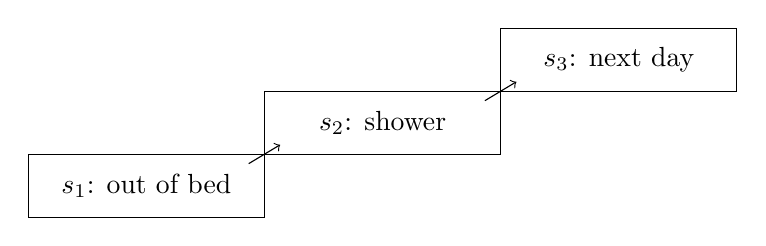
\begin{tikzpicture}[x=1cm,y=1cm]
\draw (0,0) rectangle (3,0.8);
\node at (1.5,0.4) {\(s_1\): out of bed};
\draw (3,0.8) rectangle (6,1.6);
\node at (4.5,1.2) {\(s_2\): shower};
\draw (6,1.6) rectangle (9,2.4);
\node at (7.5,2.0) {\(s_3\): next day};
\draw[->] (2.8,0.68) -- (3.2,0.92);
\draw[->] (5.8,1.48) -- (6.2,1.72);
\end{tikzpicture}
\caption{A transcript-backed staircase for Adams's ``one day at a time'' rule.}
\end{figure}

The lecture then returns from the staircase to the full burden of office. Depression is not denied. Adams names deaths, violence, and catastrophe from his first weeks as mayor. What matters is not that the burden disappears. What matters is that the office and the mission keep the next step available.

The closing beats of the interview widen once more. Cooperation across party lines is defended in practical rather than ceremonial language. Faith is stated explicitly and personally. Finally the lecture narrows into identity: be you. Those lines should remain attributed to Adams as speaker. They are not neutral textbook doctrine. Within the architecture of the lecture, however, they complete the final shift from city-scale pressure back to person-scale orientation.

\section{Summary}

This lecture gives us not one formula for wealth, but several different engines placed side by side. Russ gives us the engine of ownership: keep the master, let the catalog sum across time, and refuse early judgment. Don Vultaggio gives us the engine of cost discipline: own the assets, avoid debt, and let price and packaging carry strategic force. Rubin gives us the engine of reconstruction: study, find the void, gather the right people, ask for help, and treat failure as iteration. Adams gives us the engine of recovery under pressure: reduce the horizon to the next executable step and keep moving.

What ties these very different engines together is a single underlying law. Wealth becomes durable when the speaker controls the relevant claim. Sometimes that claim is a music catalog. Sometimes it is a debt-free factory base. Sometimes it is a network of relationships that survives bad times. Sometimes it is nothing more glamorous than the claim on the next hour of one's own life.